\chapter{Аттрактор, частично лежащий в пространстве траекторий}

\section{Пример дифференциального уравнения}

Рассмотрим дифференциальное уравнение (\cite{Vorotnikov}, remark 4.2.13, p. 97)

\begin{equation}\label{primer_iz_statyi}
	u'(t)=
	\left\{
		\begin{array}{ll}
			-(u(t)-1)^2, & u(t) > 1, \\
			-u^2 (t)   , & 0 \leq u(t) \leq 1 \\
			u^2 (t)    , & u(t) < 0
		\end{array}
	\right.
\end{equation}

и выпишем его решения и оператор сдвига.

Будем искать такие решения, что
\begin{equation}
	u(t) \in C[0; +\infty)
\end{equation}

Решим сначала каждое из трёх дифференциальных уравнений в отдельности, а затем отберём решения,
удовлетворяющие соответствующим условиям.

\begin{enumerate}

\item)
Рассмотрим обыкновенное дифференциальное уравнение
\begin{equation}\label{primer_p1}
	u'(t)=-(u(t)-1)^2
\end{equation}

Решим его как уравнение с разделяющимися переменными:
$$
	\frac{du}{dt}=-(u-1)^2
$$

Заметим, что $u\equiv 1$ --- решение уравнения (\ref{primer_p1}).
Умножив обе части на $\frac{dt}{(u-1)^2}$, имеем:
$$
	\frac{du}{-(u-1)^2}=dt
$$

Проинтегрируем обе части:
$$
	\frac{1}{u-1}=t+C
$$

Выразим $u$:
\begin{equation}\label{primer_p1_solution}
	u=\frac{1}{t+C}+1
\end{equation}
где $C\in\R$.

Заметим, что условиям $u(t) \in C[0; +\infty)$ и $u(t)>1$ удовлетворяют только решения вида (\ref{primer_p1_solution}), где $C>0$:
\begin{equation}
	u=\frac{1}{t+C}+1, C>0
\end{equation}


\item)

Рассмотрим обыкновенное дифференциальное уравнение
\begin{equation}\label{primer_p2}
	u'(t)=-u^2(t)
\end{equation}

Решим его как уравнение с разделяющимися переменными:
$$
	\frac{du}{dt}=-u^2
$$

Заметим, что $u\equiv 0$ --- решение уравнения (\ref{primer_p2}).
Умножив обе части на $\frac{dt}{u^2}$, имеем:
$$
	\frac{du}{-u^2}=dt
$$

Проинтегрируем обе части:
$$
	\frac{1}{u}=t+1+C
$$

Выразим $u$:
\begin{equation}\label{primer_p2_solution}
	u=\frac{1}{t+1+C}
\end{equation}
где $C\in\R$.

Заметим, что условиям $u(t) \in C[0; +\infty)$ и $0 \leq u(t) \leq 1$ удовлетворяют только решения вида (\ref{primer_p2_solution}), где $C\geq0$:
\begin{equation}
	u=\frac{1}{t+1+C}, C\geq0
\end{equation}
и решение $u \equiv 0$.




\item)

Рассмотрим обыкновенное дифференциальное уравнение
\begin{equation}\label{primer_p3}
	u'(t)=-u^2(t)
\end{equation}

Решим его как уравнение с разделяющимися переменными:
$$
	\frac{du}{dt}=u^2
$$

Заметим, что $u\equiv 0$ --- решение уравнения (\ref{primer_p3}).
Умножив обе части на $\frac{dt}{u^2}$, имеем:
$$
	\frac{du}{u^2}=dt
$$

Проинтегрируем обе части:
$$
	\frac{1}{u}=-(t+C)
$$

Выразим $u$:
\begin{equation}\label{primer_p3_solution}
	u=\frac{1}{-(t+C)}
\end{equation}
где $C\in\R$.

Заметим, что условиям $u(t) \in C[0; +\infty)$ и $u(t) < 0$ удовлетворяют только решения вида (\ref{primer_p3_solution}), где $C>0$:
\begin{equation}
	u=-\frac{1}{t+C}, C>0.
\end{equation}
Решение $u \equiv 0$ не удовлетворяет условию $u(t)<0$.

\end{enumerate}

Таким образом, решения уравнения (\ref{primer_iz_statyi}) выписываются в виде:
\begin{equation}\label{primer_iz_statyi_u_t}
	\left[
		\begin{array}{ll}
			u=\frac{1}{t+C}+1, & C>0
		\\\\
			u=\frac{1}{t+1+C}, & C\geq0
		\\\\
			u=0,               & C \mbox{--- любое}
		\\\\
			u=-\frac{1}{t+C},  & C>0
		\end{array}
	\right.
\end{equation}

Покажем теперь разрешимость порождаемой уравнением (\ref{primer_iz_statyi}) задачи Коши.
В силу того, что уравнение (\ref{primer_iz_statyi}) автономно, т.~е. его правая часть зависит только от $u$ и не зависит от $t$,
достаточно показать разрешимость задачи Коши с начальным условием в нуле.

Итак, пусть $u(0) = p$.
Рассмотрим четыре случая.

\begin{enumerate}

\item)
Пусть $p>1$.
Тогда по условию выпущенное из $p$ решение должно удовлетворять уравнению (\ref{primer_p1}).
Подставив $t=0$ в (\ref{primer_p1_solution}), получаем следующее уравнение для поиска $C$:
$$
	p=\frac{1}{0+C}+1
$$
Решим его:
$$
	p=\frac{1}{C}+1
$$
$$
	p-1=\frac{1}{C}
$$
$$
	C=\frac{1}{p-1}
$$
Заметим, что при $p>1$ имеем константу $C>0$, определяемую единственным образом.
Значит, решение задачи Коши при $p>1$ единственно и имеет вид:
\begin{equation}\label{primer_zk_1_0}
	u_1(t)=\frac{1}{t+\frac{1}{p-1}}+1
\end{equation}

Или, что то же самое,
\begin{equation}\label{primer_zk_1}
	u_1(t)=\frac{p+pt-t}{pt-t+1}
\end{equation}

Заметим, что из представления (\ref{primer_zk_1_0}) следует, что
$$
	\forall(p>1)\forall\left(t \in \mathbb{R}_+\right)\left[u_1(t) > 1\right],
$$
а значит, формула (\ref{primer_zk_1}) задаёт решение уравнения (\ref{primer_p1}) на всей неотрицательной полуоси $\mathbb{R}_+$.

\item)
Пусть $0<p \leq 1$.
Тогда по условию выпущенное из $p$ решение должно удовлетворять уравнению (\ref{primer_p2}).
Подставив $t=0$ в (\ref{primer_p2_solution}), получаем следующее уравнение для поиска $C$:
$$
	p=\frac{1}{0+1+C}
$$
Решим его:
$$
	C=\frac{1}{p}-1
$$
Заметим, что при $0<p \leq 1$ имеем константу $C \geq 0$, определяемую единственным образом.
Значит, решение задачи Коши при $0<p \leq 1$ единственно и имеет вид:
\begin{equation}\label{primer_zk_2_0}
	u_2(t)=\frac{1}{t+\frac{1}{p}}
\end{equation}

Или, что то же самое,
\begin{equation}\label{primer_zk_2}
	u_2(t)=\frac{p}{pt+1}
\end{equation}

Это решение снова существует на всей неотрицательной числовой полуоси $\mathbb{R}_+$, так как
$$
	\forall(0<p \leq 1)\forall\left(t \in \mathbb{R}_+\right)\left[0 < u_2(t) < 1\right].
$$

\item)
Положим теперь $p=0$.
Тогда по условию выпущенное из $p$ решение должно удовлетворять уравнению (\ref{primer_p2}).
Искомое решение есть тождественный нуль:
\begin{equation}\label{primer_zk_3}
	u_3 \equiv 0
\end{equation}
Покажем, что других решений задачи Коши нет.
Предположим противное.
Тогда решение задаётся формулой (\ref{primer_p2_solution}) и отвечает условию
$$
	0=u_{3^{'}}(0)=\frac{1}{t+1+C},
$$
правая часть которого не обращается в ноль ни при каком $C$.
Получили противоречие.
Следовательно, при $p=0$ задача Коши для исследуемого уравнения также имеет единственное решение на всей числовой полуоси $\mathbb{R}_+$.

\item)
Пусть наконец $p<0$.
Тогда по условию выпущенное из $p$ решение должно удовлетворять уравнению (\ref{primer_p3}).
Подставив $t=0$ в (\ref{primer_p3_solution}), получаем следующее уравнение для поиска $C$:
$$
	p=\frac{1}{-(0+C)}
$$
Решим его:
$$
	C=-\frac{1}{p}
$$
Заметим, что при $p<0$ имеем константу $C>0$, определяемую единственным образом.
Значит, решение задачи Коши при $p<0$ единственно и имеет вид:
\begin{equation}\label{primer_zk_4_0}
	u_4(t)=-\frac{1}{t-\frac{1}{p}}
\end{equation}

Или, что то же самое,
\begin{equation}\label{primer_zk_4}
	u_4(t)=\frac{p}{1-pt}
\end{equation}

Это решение снова существует на всей неотрицательной числовой полуоси $\mathbb{R}_+$, так как
$$
	\forall(p<0)\forall\left(t \in \mathbb{R}_+\right)\left[u_4(t) < 0\right].
$$

\end{enumerate}

\opred
Оператором сдвига $S^{t_0}_t$ по траекториям дифференциального уравнения $x'(t) = f(x,t)$ называется функция, такая, что
\begin{equation*}
	S^{t_0}_t (p) = q \Rightleftarrow
		\exists\left(x_p(t) : x_p(t_0) = p\right)\left[x_p(t) = q\right].
\end{equation*}

Т.о. оператор сдвига сдвигает точку по траектории дифференциального уравнения с момента времени $t_0$ до момента времени $t$.

\paragraph{Обозначение.}
В случае, если $t_0=0$, соответствующий оператор сдвига по траекториям дифференциального уравнения $S^{t_0}_t (p)$ в целях упрощения записи  в дальнейшем будем обозначать просто $S_t (p)$.

Учитывая (\ref{primer_zk_1})--(\ref{primer_zk_4}), оператор сдвига (в нуле) по траекториям уравнения (\ref{primer_iz_statyi}) имеет вид:
\begin{equation}\label{oper_sdviga_primer_1}
	S_t p =
	\left\{
		\begin{array}{ll}
			\frac{p+pt-t}{pt-t+1}, & p > 1
		\\\\
			\frac{p}{pt+1},        & 0 \leq p \leq 1
		\\\\
			\frac{p}{1 - pt},      & p < 0
		\end{array}
	\right.
\end{equation}


\section{Вспомогательные определения}

Дадим вспомогательные определения, которые потребуются при применении к примеру теории аттракторов,
придерживаясь [\cite{Zelenaya}, параграф 3.2].

Здесь и далее $E$ --- рефлексивное банахово пространство,
$E_0$ --- также банахово пространство и вложение $E \subset E_0$ непрерывно.
Норма в пространстве $E$ не обязательно индуцирована нормой в пространстве $E_0$.

\paragraph{Обозначение.}
В дальнейшем обозначим $T_+ = C(\mathbb{R}_+,E_0) \cap L_\infty(\mathbb{R}_+,E)$

Будем искать такие решения изучаемого дифференциального уравнения,
которые принадлежат $T_+$.


\opred
Пространством траекторий называется некоторое непустое множество $\mathcal{H}^+ \subset T_+$.

\opred
Траекторией называется элемент пространства траекторий.

При рассмотрении дифференциального уравнения под пространством траекторий мы, как это часто делается,
будем понимать множество решений этого уравнения.


\opred
Оператором сдвига $T(h)$, $h\in\R$ называется оператор, который функции $f$ ставит в соответствие функцию $T(h)f$, такую, что
$$
T(h)f(t)=f(t+h)
$$


\opred
Пространство траекторий $\mathcal{H}^+$ называется трансляционно инвариантным, если
$$
\forall(t \geq 0)\left[T(t)\mathcal{H}^+ \subset \mathcal{H}^+ \right]
$$

\opred

Пусть $B \subset T_+$.
Сечением множества траекторий $B$ в момент времени $t \geq 0$ называется множество
$$
	B(t)=\left\{u(t) : u \in B \right\} \subset E.
$$


\opred

Пусть $R,Q \subset E$.
Полуотклонением в пространстве $E_0$ множества $R$ от множества $Q$ называется величина
$$
	h_{E_0}(R,Q) = \sup_{r\in R} \inf_{q \in Q} \| q - r \|_{E_0}.
$$

Заметим, что полутклонение --- не симметричная операция.
Приведём пример случая, когда
$$
	h_{E_0}(R,Q) \neq h_{E_0}(Q,R),
$$
являющийся частным случаем примера [\cite{mnogozn}, теорема 1.2.41].

Пусть $E_0 = E = \mathbb{R}$, $\|x\|_{\mathbb{R}} = |x|$,
$$
	R =\{0\},
$$
$$
	Q=\{0;1\}.
$$
Тогда
\begin{multline*}
	h_{E_0}(R,Q) =
	\sup_{r\in R} \inf_{q \in Q} \| q - r \|_{E_0} =
	\sup_{r\in \{0\}} \inf_{q \in \{0;1\}} | q - r | =
	\inf_{q \in \{0;1\}} | q - 0 | =
	\\ =
	\min\{|0-0|,|1-0|\} =
	\min\{0;1\} =
	0;
\end{multline*}
с другой стороны,
\begin{multline*}
	h_{E_0}(Q,R) =
	\sup_{q \in Q} \inf_{r\in R} \| r - q \|_{E_0} =
	\sup_{q \in \{0;1\}} \inf_{r\in \{0\}} | r - q | =
	\sup_{q \in \{0;1\}} | 0 - q | =
	\\ =
	\max\{|0-0|,|0-1|\} =
	\max\{0;1\} =
	1.
\end{multline*}
Т.е.
$$
	h_{\mathbb{R}}\left( \{0\}, \{0;1\}\right) \neq h_{\mathbb{R}}\left( \{0;1\} , \{0\} \right).
$$


\section{Аттрактор полугруппы трансляций (динамической системы)}

Перейдём теперь к центральному понятию, рассматриваемому в данной работе --- понятию аттрактора.

Название <<аттрактор>> (англ. <<attractor>>) буквально означает <<притягивающий>>.



Введём теперь понятие аттрактора полугруппы, следуя [\cite{Vorotnikov}, \S 4.1.1],
и покажем, что в рассматриваемом примере аттрактора полугруппы трансляций нет.

\opred

Семейство отображений $S_t : E \to E$, $t \geq 0$ называется полугруппой трансляций,
если $S_0$ --- тождественное отображение и
$$
	\forall(t>0,\tau>0)[S_t \circ S_\tau = S_{t+\tau}]
$$

Здесь и далее под $E$ будем понимать банахово пространство.

\opred

Полугруппа $S_t$ называется ограниченной в $E$, если для любого ограниченного в $E$ множества $B \subset E$ множество $\bigcup\limits_{t\geq0}S_t B$ также ограничено в $E$.

Здесь и далее через $F$ будем обозначать топологическое пространство, такое, что $E \cap F \ne \varnothing$.

\opred

Множество $A$ называется инвариантным относительно полугруппы трансляций $S_t$, если
$$
	\forall(t\geq 0)[S_t A = A]
$$

\opred

Множество $P \subset F$ называется $(E,F)$-притягивающим для полугруппы трансляций $S_t$,
если для любого ограниченного множества $B \subset E$ и любой открытой окрестности $W$ множества $P$ в $F$ существует число $h\geq 0$ такое, что
$$
	\forall(t \geq h)[S_t B \subset W]
$$


\opred

Множество $A\subset E\cap F$ называется $(E,F)$-аттрактором полугруппы трансляций $S_t$, если

а) $A$ компактно в $F$ и ограничено в $E$;

б) $A$ инвариантно относительно полугруппы трансляций $S_t$.

в) $A$ является $(E,F)$-притягивающим для полугруппы трансляций $S_t$.

Часто аттрактор полугруппы трансляций называют аттрактором динамической системы.

Возвращаясь к разбираемому примеру, попробуем применить только что данное определение к полугруппе трансляций (\ref{oper_sdviga_primer_1}).

(\ref{oper_sdviga_primer_1}) --- действительно полугруппа трансляций, т.к. явно задано $S_0 p = p$, а равенство $S_t \circ S_\tau = S_{t+\tau}$ следует из автономности дифференциального уравнения.

Очевидно, что $E=F=\mathbb{R}$.

Покажем, что у полугруппы трансляций (\ref{oper_sdviga_primer_1}) нет $(\mathbb{R},\mathbb{R})$-аттрактора.

Предположим противное.
Пусть такой аттрактор $A \subset \mathbb{R}$ существует.
Тогда $A$ должно быть инвариантно относительно полугруппы трансляций $S_t$ и компактно в $\R$, следовательно, и замкнуто в $\R$.
Используя запись (\ref{oper_sdviga_primer_1}), легко найти, что
\begin{equation}\label{oper_sdviga_primer_1_proizv}
	\frac{d}{dt}S_t p =
	\left\{
		\begin{array}{ll}
			\frac{-(p-1)^2}{(pt-t+1)^2} < 0, & p > 1
		\\\\
			0,        & p = 0
		\\\\
			\frac{-p^2}{(pt+1)^2} < 0,        & 0 < p \leq 1
		\\\\
			\frac{-p}{1 - pt} > 0,      & p < 0
		\end{array}
	\right.
\end{equation}

Так как множество $A$ замкнуто в $\R$, то оно содержит свои минимум и максимум.

Пусть $m = \min A < 0$.
Тогда в силу (\ref{oper_sdviga_primer_1_proizv}) $S_1 m > m$, следовательно, $m \notin S_1 A$ и $S_1 A \neq A$.
Следовательно, $m \geq 0$.
Но тогда и $M = \max A \geq 0$.

Пусть $M > 0$.
В силу (\ref{oper_sdviga_primer_1_proizv}) $S_1 M < M$, следовательно, $M \notin S_1 A$ и $S_1 A \neq A$.

Значит, $M=m=0$, т.е. $A=\{0\}$.
Покажем, что в таком случае множество $A$ не является $(\R,\R)$-притягивающим для полугруппы трансляций $S_t$, а следовательно, не является $(\R,\R)$-аттрактором для полугруппы трансляций $S_t$.

Действительно, для множества $A$ рассмотрим его открытую окрестность $ W = (-\frac12;\frac12)$.
Положим $B_2={2}$.
Очевидно, что $B_2$ ограничено в $\R$.
Тогда из (\ref{oper_sdviga_primer_1}) и (\ref{oper_sdviga_primer_1_proizv}) следует, что
$$
	\forall(t>0)[S_t B_2 \subset [1; 2]],
$$
но $[1;2]\cap W = \varnothing$, откуда
$$
	\forall(t>0)[S_t B_2 \not\subset W],
$$

т.е. $A$ не является $(\R,\R)$-притягивающим для полугруппы трансляций $S_t$,
а значит, и $(\R,\R)$-аттрактором для $S_t$.

Таким образом, мы доказали, что у полугруппы трансляций, заданной соотношением (\ref{oper_sdviga_primer_1}),
нет $(\R,\R)$-аттрактора.

Покажем теперь, что теория минимальных траекторных аттракторов и глобальных аттракторов
даёт для этого примера наличие траекторного и глобального аттракторов.


\section{Минимальный траекторный аттрактор}

Покажем, что минимальный траекторный аттрактор существует, и найдём его.

\opred (\cite{zhidkosti_s_pamyatyu}, опр. 2; \cite{Zelenaya}, параграф 3.2, стр. 122, опр. 3.2.2; предл. 3.2.1)

Множество $P \subset T_+$ называется притягивающим для пространства траекторий $\mathcal{H}^+$ в топологии пространства $C(\mathbb{R}_+; E_0)$,
если для всякого множества $B \subset \mathcal{H}^+$, ограниченного в $L_{\infty}(\mathbb{R}_+;E)$, выполняется условие
\begin{equation}
	h_{E_0}(B(t),T(t)P) \xrightarrow[t\to\infty]{}0
\end{equation}

\opred (\cite{Zelenaya}, опр. 4.1.5; \cite{zhidkosti_s_pamyatyu}, опр. 3)

Непустое множество $\mathcal{U}\subset T^+$
называется траекторным аттрактором для пространства траекторий $\mathcal{H}^+$
относительно топологии $C(\mathbb{R}_+,E_0)$, если
\begin{enumerate}
	\item)
		$\mathcal{U}$ компактно в $C(\mathbb{R}_+,E_0)$;
	\item)
		$\mathcal{U}$ ограничено в $L_{\infty}(\mathbb{R}_+,E)$;
	\item)
		$\mathcal{U}$ трансляционно инвариантно;
	\item)
		$\mathcal{U}$ является притягивающим для пространства траекторий $\mathcal{H}^+$
		в топологии пространства $C(\mathbb{R}_+; E_0)$.
\end{enumerate}

\opred (\cite{zhidkosti_s_pamyatyu}, опр. 3)
Минимальным траекторным аттрактором пространства траекторий $\mathcal{H}^+$
называется такой траекторный аттрактор, который содержится в любом другом траекторном аттракторе.


Покажем наконец, что для уравнения (\ref{primer_iz_statyi}) минимальный траекторный аттрактор имеет вид
\begin{equation}
	P = \{ v_0(t) \equiv 0, v_1(t) \equiv 1\}
\end{equation}

Покажем сначала, что $P$ --- траекторный аттрактор.

Очевидно, что конечное множество $P$ и компактно, и ограничено в любых пространствах.
Трансляционная инвариантность функций, тождественно равных константе, также очевидна.

Для доказательства того, что $P$ --- траекторный аттрактор осталось доказать,
что $P$ --- притягивающее множество для пространства траекторий $\mathcal{H}^+$ в топологии пространства $C(\mathbb{R}_+; E_0)$.

Пусть $Q \subset \mathcal{H}^+$ --- ограниченное в $L_{\infty}(\mathbb{R}_+;E)$ множество.
Тогда
\begin{equation}
	\exists(K>0)\forall(u\in Q)\left[ \| u \|_{L_{\infty}(\mathbb{R}_+;E)} < K\right]
\end{equation}
т.е., с учётом того, что
$$
	\| u \|_{L_{\infty}(\mathbb{R}_+;E)} = \sup_{t\geq 0}|u(t)|
$$
получаем, что
\begin{equation}
	\exists(K>0)\forall(u\in Q)\forall(t \geq 0)\left[ | u (t) | < K\right]
\end{equation}
и, в частности,
\begin{equation}
	\exists(K>0)\forall(u\in Q)\left[ | u (0) | < K\right]
\end{equation}

Положим $K>1$ и зафиксируем константу $K$.

Пусть решение имеет вид (\ref{primer_p1_solution}).
Тогда в выражении $u_1(t)=\frac{1}{t+\frac{1}{p-1}}+1$  (см. (\ref{primer_zk_1_0})) $1<p<K$ и
\begin{multline}
	|u_1(t) - v_1(t)| =
	|u_1(t) - 1| =
	\left|\left(\frac{1}{t+\frac{1}{p-1}}+1\right) -1\right| =
	\\ =
	\left|\frac{1}{t+\frac{1}{p-1}}\right| \leq
	\left|\frac{1}{t}\right| =
	\frac{1}{t}
	\xrightarrow[t\to+\infty]{}0
\end{multline}

Пусть решение имеет вид (\ref{primer_p2_solution}).

Тогда в выражении $u_2(t)=\frac{1}{t+\frac{1}{p}}$  (см. (\ref{primer_zk_2_0})) $0 < p \leq 1 < K$ и
\begin{equation}
	|u_2(t) - v_0(t)| =
	|u_2(t) - 0| =
	|u_2(t)| =
	\left| \frac{1}{t+\frac{1}{p}} \right| \leq
	\left|\frac{1}{t}\right| =
	\frac{1}{t}
	\xrightarrow[t\to+\infty]{}0
\end{equation}

Случай, когда решение имеет вид $u_3(t) \equiv 0$, тривиален.

Пусть, наконец, решение имеет вид (\ref{primer_p3_solution}).

Тогда в выражении $u_4(t)=-\frac{1}{t-\frac{1}{p}}$  (см. (\ref{primer_zk_4_0})) $-K < p < 0$ и
\begin{multline}
	|u_4(t) - v_0(t)| =
	|u_4(t) - 0| =
	|u_4(t)| =
	\left| -\frac{1}{t-\frac{1}{p}} \right| =
	\\ =
	\left| \frac{1}{t+\frac{1}{-p}} \right| \leq
	\left|\frac{1}{t}\right| =
	\frac{1}{t}
	\xrightarrow[t\to+\infty]{}0
\end{multline}

Заметим, что в данном примере стремление функций $u_1$, $u_2$, $u_3$ и $u_4$ к соответствующим функциям из траекторного аттрактора не зависит от выбора константы $K$: функции мажорируются гиперболами.

Следовательно,
\begin{multline}
	h_{\mathbb{R}}(Q(t),P(t)) =
	\sup_{u\in Q} \inf_{v_i \in P} |u(t) - v_i(t)| =
	\\ =
	\sup_{u\in Q} \min(|u(t) - v_0(t)|,|u(t) - v_1(t)|) \leq
	\sup_{u\in Q} \frac{1}{t} =
	\frac{1}{t}
	\xrightarrow[t\to+\infty]{}0
\end{multline}

Таким образом, множество $P$ действительно является притягивающим для пространства траекторий $\mathcal{H}^+$ уравнения (\ref{primer_iz_statyi}) и, с учётом выше, является траекторным аттрактором.

Покажем, что $P$ --- минимальный траекторный аттрактор.
Предположим противное.
Тогда либо $P_0 =\{v_0(t) \equiv 0\}$, либо $P_1 =\{v_1(t) \equiv 1\}$ также является траекторным аттрактором.
Но $P_1$ --- не траекторный аттрактор, т.к. для решения $u_3(t) \equiv 0$ имеем
\begin{equation}
	h_{\mathbb{R}}(\{u_3(t) \equiv 0 \},P_1(t)) =
	|u_3(t) - v_1(t)| =
	|0-1| =
	1
	%\not{\xrightarrow[t\to+\infty]{}0}
\end{equation}

Аналогично траекторным аттрактором не является $P_0$.
Действительно, для решения вида $u_1(t)=\frac{1}{t+\frac{1}{p-1}}+1, p > 1$ имеем

\begin{multline}
	h_{\mathbb{R}}(\{u_1(t)\},P_0(t)) =
	|u_1(t) - v_0(t)| =
	|u_1(t) - 0| =
	\\ =
	|u_1(t)| =
	\left| \frac{1}{t+\frac{1}{p-1}}+1 \right| =
	\frac{1}{t+\frac{1}{p-1}}+1 >	1
	%\not{\xrightarrow[t\to+\infty]{}0}
\end{multline}

Следовательно, траекторный аттрактор $P$ --- минимальный.
Примечательно, что функция $v_1(t) \equiv 1$ принадлежит минимальному траекторному аттрактору,
но не принадлежит пространству траекторий.


\section{Глобальный аттрактор}

Пусть $E\subset E_0$ --- те же, что и указано выше.

\opred (\cite{Zelenaya}, параграф 3.2, стр. 121-122, опр. 3.2.1)

Множество  $\mathcal{A} \subset E $ называется глобальным аттрактором (в $E_0$) для пространства траекторий $\mathcal{H}^+$, если:
\begin{enumerate}
	\item)
		$\mathcal{A}$ компактно в $E_0$ и ограничено в $E$;
	\item)
		для любого ограниченного в $L_\infty(\mathbb{R}_+; E)$ множества $X \subset \mathcal{H}^+$
		выполнено условия притягивания
		$$
			h_{E_0}(X(t),\mathcal{A}) \xrightarrow[t\to \infty]{}{0}.
		$$
	\item)
		$\mathcal{A}$ --- наименьшее по включению множество, удовлетворяющее условиям (1) и (2).
\end{enumerate}


Глобальный аттрактор, как следует из определения, принадлежит фазовому пространству.
Глобальный аттрактор представляет собой набор состояний, к которым система будет стремиться со временем;
все остальные состояния системы, т.е. точки фазового пространства, не входящие в глобальный аттрактор, преходящи;
с учётом того, что в реальных измерениях всегда присутствует некоторая погрешность, тем фактом, что решения могут не достигать глобального аттрактора, а только приближаться к нему, можно пренебречь и изучать только состояния системы, соответствующие глобальному аттрактору.

Существование глобального аттрактора дл данного примера непосредственно следует из существования
минимального траекторного аттрактора и [\cite{Zelenaya}, теорема 4.4.1].
Эта теорема утверждает, что глобальный аттрактор явлется сечением минимального траекторного аттрактора.
В силу трансляционной инвариантности минимального траекторного аттрактора безразлично,
в какой именно момент времени брать его сечение.

Выше мы доказали, что минимальным траекторным аттрактором является множество $P=\{v_0(t)\equiv 0; v_1(t)\equiv 1\}$.
Следовательно, глобальным аттрактором явлется множество $G = P(t) = \{0; 1\}$.

\chapter{Минимальный траекторный аттрактор, целиком лежащий вне пространства траекторий}

\section{Минимальный траекторный аттрактор}

\begin{wrapfigure}[30]{r}{6cm}
	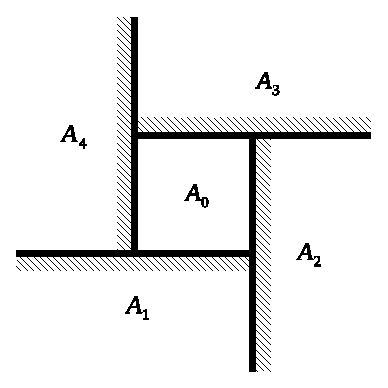
\includegraphics[width=\linewidth]{quad2-1.eps}
	\caption{Разбиение плоскости}
	\label{fig:somelabel}
	%\vspace{2cm}
\end{wrapfigure}

Положим $E=E_0=\R^2$.
Разобьём $\R^2$ на пять непересекающихся связных множеств следующим образом:
$$
	A_0 = \{ (x_1, x_2) \mid 0 < x_1 < 1,~~ 0 < x_2 < 1\}
$$
$$
	A_1 = \{ (x_1, x_2) \mid x_1 < 1,~~ x_2 \leq 0  \}
$$
$$
	A_2 = \{ (x_1, x_2) \mid x_1 \geq 1,~~ x_2 < 1  \}
$$
$$
	A_3 = \{ (x_1, x_2) \mid x_1 > 0,~~ x_2 \geq 1  \}
$$
$$
	A_4 = \{ (x_1, x_2) \mid x_1 \leq 0,~~ x_2 > 0  \}
$$
и отметим точки
$\alpha_1=(1, 0)$,
$\alpha_2=(1, 1)$,
$\alpha_3=(0, 1)$ и
$\alpha_4=\alpha_0=(0, 0)$
(двойное обозначение используется для удобства работы с индексами).

Сразу заметим, что $\alpha_i \in \overline{A_i}$, $i=0,...,4$ и
$\alpha_i \in A_{i+1}$, $i=0,...,3$ (тогда как $\alpha_4 = \alpha_0 \in A_{1}$).

Таким образом, вся координатная плоскость оказалась разбита на четыре угла $A_1, ..., A_4$ и квадрат $A_0$.
Квадрат не включает свои границы; для каждого угла одна его сторона включается в угол,
а вторая сторона и вершина --- нет (они включаются в <<соседний>>).
Именно за счёт такого разбиения и достигается эффект примера.

В дальнейшим первый нижний индекс будет отвечать за номер области и обозначаться через $i$,
$i=0, ..., 3$, второй --- за координату и обозначаться $j$, $j=1, 2$.

Рассмотрим дифференциальное уравнение
\begin{equation}\label{difur_primer_R2}
	\frac{dx_j(t)}{dt} = -\gamma_{ij}(x_j(t)-p_{ij})^2,
\end{equation}
где
$$
	\gamma_{ij} = \sgn(x_j(0)-p_{ij}),~~j=1,2;~~~~
	(x_1, x_2) \in A_i, ~~~ \alpha_i = (p_{i1},p_{i2}).
$$

Де-факто это --- система из двух дифференциальных уравнений, по одному уравнению на координату.
Обратим внимание, что каждая координата меняется независимо от другой и гиперболически стремится
к некоторому предельному значению (это будет показано далее).

Для удобства решения представим это уравнение в виде
\begin{equation*}
	\frac{d(x_j(t) - p_{ij})}{dt} = -\gamma_{ij}(x_j(t)-p_{ij})^2,
\end{equation*}
т.е. добавим константу под знаком дифференциала.

Если $\gamma_{ij} = 0$, то $x_j(t) \equiv const$.
Если $\gamma_{ij} \neq 0$, то разделим переменные $t$ и $(x_j(t) - p_{ij})$:
\begin{equation*}
	\frac{d(x_j(t) - p_{ij})}{-\gamma_{ij}(x_j(t)-p_{ij})^2} = dt ,
\end{equation*}
откуда
\begin{equation*}
	\frac{\gamma_{ij}}{x_j(t)-p_{ij}} = t+C_0, C_0 > 0
\end{equation*}
(неравенство на $C_0$ налагается для обеспечения существования решения на всей положительной полуоси),
или, что то же самое,
\begin{equation}\label{primer_R2_x_j}
	x_j(t) = \frac{\gamma_{ij}}{t+C_0}+p_{ij}, C_0 > 0
\end{equation}
откуда
\begin{equation*}
	x_j(t) \xrightarrow[t\to \infty ]{}{p_{ij}},
\end{equation*}
при этом знак разности $x_j(t) - p_{ij}$ не меняется.
Заметим, что формула (\ref{primer_R2_x_j}) верна и для случая $\gamma_{ij}=0, x_j(0)=p_{ij}$.

\begin{wrapfigure}[18]{r}{7.5cm}
	%\vspace{-5ex}
	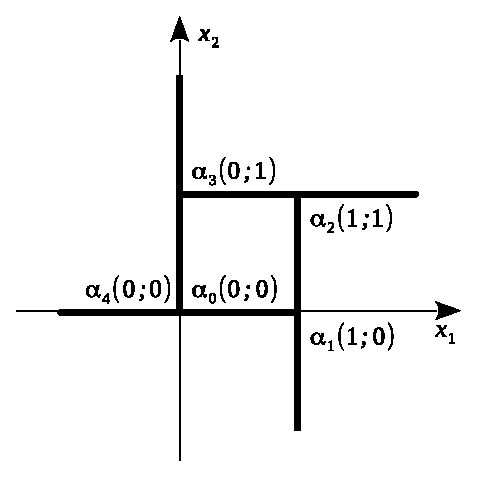
\includegraphics[width=\linewidth]{quad2-2.eps}
	\caption{Отмеченные точки}
	\label{fig:somelabel2}
\end{wrapfigure}

Выпишем теперь оператор сдвига.
Положим в (\ref{primer_R2_x_j}) $t=0$, получим
$$
	x_j(0) = \frac{\gamma_{ij}}{C_0}+p_{ij}
$$
Таким образом, оператор сдвига по траекториям уравнения (\ref{difur_primer_R2}) имеет вид
\begin{equation}\label{primer_R2_oper_sdviga}
	\tilde{S}_t(x_{j0}) = \frac{x_{j0}-p_{ij}}{|x_{j0}-p_{ij}|t+1}+p_{ij}
\end{equation}

Для $x_0 \in A_i$ имеем
\begin{equation}\label{primer_R2_stremlenie}
	S_t(x_0) \xrightarrow[t \to \infty]{} \alpha_{i},
\end{equation}
причём монотонно по $t$.
Действительно,
\begin{multline}
	\|S_t(x_0) - \alpha_i\| \leq
	\sqrt{2} \max_{j=1,2} \left| \frac{x_{j0}-p_{ij}}{|x_{j0}-p_{ij}|t+1} + p_{ij} - p_{ij}  \right| = \\ =
	\sqrt{2} \max_{j=1,2} \left| \frac{x_{j0}-p_{ij}}{|x_{j0}-p_{ij}|t+1} \right| \leq
	\sqrt{2} \max_{j=1,2} \left| \frac{x_{j0}-p_{ij}}{|x_{j0}-p_{ij}|t} \right| =
	\\ =
	\sqrt{2} \max_{j=1,2} \left| \frac{1}{t} \right| =
	\frac{\sqrt{2}}{t} \xrightarrow[t \to \infty]{} 0
\end{multline}

Заметим, что эта оценка равномерна по $x_{j0}$.
Более того, из того, что $\alpha_i \in A_{i+1}$, $i=0,...,3$,
следует, что $S_t(\alpha_i) \xrightarrow[t \to \infty]{} \alpha_{i+1}$,
т.е. множество функций-констант
$$
	U = \{ u_i(t) \equiv \alpha_i \}_{i=0}^{3}
$$
не пересекается со множеством решений уравнения (\ref{difur_primer_R2}).

Покажем теперь, что $U$ --- траекторный аттрактор в смысле [\cite{Zelenaya}, опред. 3.2.3].
Компактность и ограниченность множества из четырёх функций-констант в пространствах
$C(\R_+; \R^2)$ и $L_\infty(\R_+; \R^2)$ очевидна.
Очевидно и то, что $U$ трансляционно инвариантно.

Осталось показать, что $U$ есть притягивающее множество в пространстве траекторий $H^+$ уравнения (\ref{difur_primer_R2}).
Действительно, пусть $M>0$ и $B\subset H^+$ --- ограниченное в $L_\infty(\R_+; \R^2)$ множество.
Тогда
\begin{multline*}
	h_{C([0,M];\R^2)}(\Pi_M T(t)B,\Pi_M U) =
	\\ =
	\sup_{v\in B} \inf_{u\in U} \| T(t) v - u \|_{C([0,M];\R^2)} =
	\sup_{v\in B} \min_{i=0,..,3} \| T(t) v - u_i \|_{C([0,M];\R^2)} =
	\\ =
	\sup_{v\in B} \min_{i=0,..,3} \max_{s\in[0,M]} \| (T(t) v)(s) - u_i(s) \| =
	\sup_{v\in B} \min_{i=0,..,3} \max_{s\in[0,M]} \| (T(t) v)(s) - \alpha_i \| =
	\\ =
	\sup_{v\in B} \min_{i=0,..,3} \max_{s\in[t,t+M]} \| v(s) - \alpha_i \| \leq
	\frac{\sqrt{2}}{t} \xrightarrow[t\to + \infty]{} 0
\end{multline*}
Таким образом, $U$ --- действительно траекторный аттрактор, пересечение которого с пространством траекторий
уравнения (\ref{difur_primer_R2}) пусто.

\begin{wrapfigure}[14]{r}{7.5cm}
	%\vspace{-5ex}
	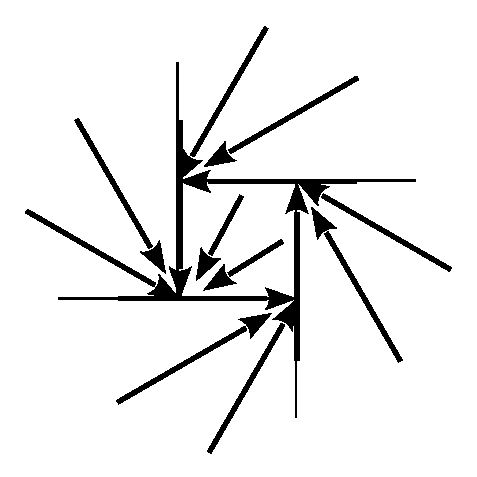
\includegraphics[width=\linewidth]{quad2-3.eps}
	\caption{Направления сдвигов}
	\label{fig:somelabel3}
\end{wrapfigure}

\section{Аттрактор полугруппы трансляций (динамической системы)}

Покажем теперь, что $(\mathbb{R}^2,\mathbb{R}^2)$--аттрактора полугруппы трансляций в данном примере не существует.
Предположим противное, т.е. что существует $P$ --- аттрактор полугруппы трансляций,
порождаемой оператором сдвига (\ref{primer_R2_oper_sdviga}).

Пусть сначала $\exists(i=0,...,4)[\alpha_i \notin P]$.
Тогда в силу условия (а) из определения аттрактора полугруппы трансляций вытекает,
что $A$ --- компактно в $\mathbb{R}^2$.
Тогда расстояние $\rho$ от $P$ до $\alpha_i$ положительно.

Положим $\varepsilon = \frac{\rho}{3} > 0$ и покажем,
что условие притяжения из определения аттрактора полугруппы трансляций не выполняется.

Рассмотрим $V_\varepsilon = A_i \cap B(\alpha_i, \varepsilon)$ и некоторое решение $x_\varepsilon(t)$
такое, что $x_\varepsilon(0) \in V_\varepsilon$.
Тогда в силу монотонности стремления (\ref{primer_R2_stremlenie})
$\forall(t>0)[x_\varepsilon(t) \in V_\varepsilon]$.
Но $V_\varepsilon$ отделено от $P$, следовательно, $x_\varepsilon{t}$ не попадает в $\varepsilon$--окрестность $P$
ни при каких положительных $t$, что доказывает нарушение условия притяжения.

Значит, если аттрактор $P$ полугруппы трансляций существует, то $\alpha_i \in P, i=0,...,4$.
Но тогда $\forall(t>0)[S_t P \ne P]$.
Действительно, траектория, выходящая из $\alpha_i$, стремится к $\alpha_{i+1}$;
а все траектории, выходящие из точек области $A_i$, стремтся к $\alpha_i$,
но никогда не достигают её.

Следовательно, аттрактора полугруппы трансляций в данном случае не существует.




\addcontentsline{toc}{chapter}{Литература}
\begin{thebibliography}{99}

\bibitem{Vorotnikov} Topological Approximation Methods for Evolutionary Problems of Nonlinear Hydrodynamics / Victor G. Zvyagin, Dmitry A. Vorotnikov. Walter de Gruyter, Berlin, New York. 2008.

\bibitem{Kondratyev} Аттракторы уравнений неньютоновской гидродинамики / В. Г. Звягин, С. К. Кондратьев. – Успехи математических наук, 2014, сентябрь-октябрь, т. 69, вып 5 (419). – 76с.

\bibitem{Fursikov} Оптимальное управление распределёнными системами. Теория и приложения / А. В. Фурсиков. Новосибирск. Научная книга, 1999.

\bibitem{mnogozn} Введение в теорию многозначных отображений и дифференциальных включений / Ю. Г. Борисович, Б. Д. Гельман, А. Д. Мышкис, В. В. Обуховский.  2е изд., ЛИБРОКОМ, М., 2011. – 224с.

\bibitem{Zelenaya} Аттракторы для уравнений моделей движения вязкоупругих сред : учебное пособие / В.\,Г.\,Звягин, С.\,К.\,Кондратьев~; Воронежский государственный университет. -- Воронеж : Издательско-полиграфический центр Воронежского государственного университета, 2010. --- 266 с.

\bibitem{zhidkosti_s_pamyatyu} Аттракторы слабых решений регуляризованной системы уравнений движения жидких сред с памятью / В.\,Г.\,Звягин, С.\,К.\,Кондратьев~; Известия вузов: Математика, 2011, № 8 --- c. 86–89

\end{thebibliography}
